%% LyX 2.2.3 created this file.  For more info, see http://www.lyx.org/.
%% Do not edit unless you really know what you are doing.
\documentclass[english]{article}
\usepackage[T1]{fontenc}
\usepackage[latin9]{inputenc}
\usepackage{geometry}
\geometry{verbose,lmargin=2cm,rmargin=2cm}
\usepackage{babel}
\usepackage{float}
\usepackage{graphicx}
\usepackage[unicode=true,pdfusetitle,
 bookmarks=true,bookmarksnumbered=false,bookmarksopen=false,
 breaklinks=false,pdfborder={0 0 1},backref=false,colorlinks=false]
 {hyperref}
\usepackage{breakurl}

\makeatletter

%%%%%%%%%%%%%%%%%%%%%%%%%%%%%% LyX specific LaTeX commands.
%% Because html converters don't know tabularnewline
\providecommand{\tabularnewline}{\\}
%% A simple dot to overcome graphicx limitations
\newcommand{\lyxdot}{.}

\floatstyle{ruled}
\newfloat{algorithm}{tbp}{loa}
\providecommand{\algorithmname}{Algorithm}
\floatname{algorithm}{\protect\algorithmname}

\makeatother

\usepackage{listings}
\renewcommand{\lstlistingname}{Listing}

\begin{document}

\title{Classifying Books By Writing Style Using Machine Learning Techniques\thanks{This project was done within the frame of the machine learning course
(COMS3007) held at the University of the Witwatersrand in 2018}}

\author{By:\\
Or Hanoch (1501858)\\
 Devon Jarvis (1365149)\\
Meir Rosendorff (1490527)\\
Kimessha Paupamah (1038238)\\
Instructor:\\
Dr. Benjamin Rosman}

\maketitle
\setcounter{section}{-1}
\section{Introduction}

In this project we use different machine learning techniques learnt
in the course to recognize which book, from a set of books, a given
page is from. In particular we were interested in doing this with
the seven Harry Potter books in order to see if there is any distinguishable
change in writing style as the series progressed.

We used the following techniques:
\begin{itemize}
\item Na�ve Bayes
\item k-Means clustering
\item Neural Networks
\end{itemize}
We used these techniques on both the Harry Potter series of books
and on a general benchmark set of 7 books from different genres. We
used the general benchmark test to asses our algorithms and see if
the results we obtained from the Harry Potter set were due to J.K
Rowling's change in writing over time or if it was due to our algorithms
being problematic and not suiting this particular problem well. The
benchmark set of books included: 
\begin{itemize}
\item Book1 - The Old Testament (Religion)
\item Book2 - A Natural History of Ducks (History)
\item Book3 - Lord of the Rings - all 3 books merged into 1 (Fantasy)
\item Book4 - Fifty Shades of Grey (Romance)
\item Book5 - 1922 (Horror)
\item Book6 - Macbeth (Shakespearian Novel)
\item Book7 - The Adventures of Sherlock Holmes (Crime/Detective)
\end{itemize}
The process and results are specified below.

\section{Na�ve Bayes}

\subsection{Background}

The Na�ve Bayes Algorithm uses a list of probabilities and Bayes Rule
to classify data into groups. The idea of this project was to classify
sets of pages from the Harry Potter books into the books in which
they belong.

\subsection{Methods}

\subsubsection{Data Pre-Processing }

We start off by splitting all the books into page sets (We will explain
later how we optimized the `pageSetSize` which is the number of pages
in a set). We then took around 20\% of these from each book and set
them aside for validation data which we used for training our hyper-parameters,
we set a further 20\% aside for testing and the remaining 60\% we
used for training data. \\

We removed all punctuation from the data, except for question marks
and exclamation marks which were separated into their own words as
we felt this may give more insight as J.K. Rowling may have asked
more questions or written more exclamations in some books than others.\\

We then took our training data and we calculated the probability for
each word appearing in any one page set from each book. We did this
by counting the number of page sets a word appears in in each book
and dividing it by the total number of page sets in that book. This
gave us our probability tables, each of which contain probabilities
for around 20 000 words. Each of the tables contains a different number
of words because of how the data is split up and which data the trainer
sees and which is used for testing (see folder probTables where we
have stored each of our tables). 

In order to narrow down our dictionary (to improve both speed and
accuracy) we decided to remove common words that don\textquoteright t
differentiate well between books. We did this by comparing the probabilities
for each word of it appearing in each book and if at least one of
these seven probabilities where greater than `upperThreshold` and
at least `requiredNum` probabilities are less than `lowerThreshold`
we then kept the word. By doing this we only keep words that appear
often in one or more books and barely appear in multiple other books. 

Using the validation data we optimized the hyperparameters: `pageSetSize`,
`upperThreshold`, `lowerThreshold` and `requiredNum`. We did this
using the following algorithm: 

\begin{algorithm}
\caption{Na�ve Bayes - Keeping Relevant Words}

\begin{lstlisting}[language=Octave]
for each set of pages do
	create probability table based off size of page set using trainingData
end for
for each requiredNum in range 1 - 5 do

	currTable = probailityTable with words removed based off
				upperThreshold, lowerThreshold and requiredNum
	while accuracy on validation data is improving do

		while accuracy on validation data is improving do

			Decrease lowerThreshold by alpha
			currTable = probailityTable with words removed based off
						new upperThreshold, lowerThreshold and requiredNum
			Retest on validation data 
		end while

		while accuracy on validation data is improving do
			Increase upperThreshold by alpha
			currTable = probailityTable with words removed based off
						new upperThreshold, lowerThreshold and requiredNum
			Retest on validation data 
		end while

		Change alpha by a factor of a half
		If alpha is less than a threshold exit the loop
	end while
end for
take the pageSetSize, upperThreshold, lowerThreshold and requiredNum
that yield the best accuracy

test on testing data
\end{lstlisting}
\end{algorithm}

\subsubsection{Na�ve Bayes Procedure}

\subsubsection{Hyper-Perameter Tuning}

\subsection{Results}

The following graph shows the accuracy given for the different pageSetSizes
on our test data, it should be noted that since there are 7 options
a random guess will be correct 14.29\% of the time.

\includegraphics{naive_bayes/Project/Images/new_accuracy\lyxdot PNG}\\
It is quite clear a pageSetSize of 5 gives the highest accuracy. Since
the pageSetSize of 5 gives the highest accuracy, we use this pageSetSize
in our analysis.\\
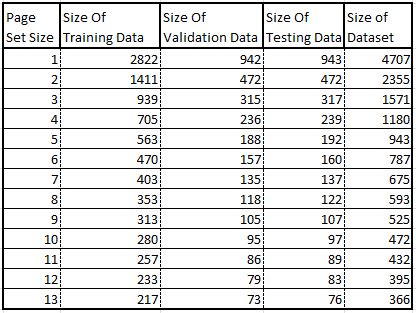
\includegraphics{naive_bayes/Project/Images/pageSetSizeTable}\\
Thus the best classifier that we found was trained using the following
parameters: 
\begin{itemize}
\item pageSetSize = 5
\item Training pageSets = 563 
\item Testing pageSets = 192
\item Validation pageSets = 188 
\item Words Used for Classifying = 1594 
\item requiredNum = 1 
\item upperThreshold = 0.051875 
\item lowerThreshold = 0.03125
\end{itemize}

\subsubsection{Confusion Matrix}

The following is the confusion matrix we got after testing this classifier
on 317 test cases

\begin{tabular}{|c|c|c|c|c|c|c|c|}
\hline 
 & 1 & 2 & 3 & 4 & 5 & 6 & 7\tabularnewline
\hline 
\hline 
1 & 12 & 2 & 1 & 0 & 2 & 0 & 0\tabularnewline
\hline 
2 & 1 & 13 & 1 & 0 & 0 & 0 & 0\tabularnewline
\hline 
3 & 1 & 0 & 15 & 2 & 2 & 0 & 0\tabularnewline
\hline 
4 & 0 & 0 & 0 & 27 & 1 & 0 & 1\tabularnewline
\hline 
5 & 0 & 1 & 2 & 3 & 36 & 1 & 0\tabularnewline
\hline 
6 & 0 & 0 & 1 & 1 & 2 & 26 & 1\tabularnewline
\hline 
7 & 0 & 0 & 0 & 0 & 2 & 3 & 32\tabularnewline
\hline 
\end{tabular}

This confusion matrix has an accuracy of 83.85\%. There a quite a
few interesting observations that can be made about the harry potter
books from this matrix. The first thing that jumps out as obvious
in this matrix (and is reflected in all the others) is an obvious
bias to book 5 and book 7.

\includegraphics{naive_bayes/Project/Images/new_classification\lyxdot PNG}

This could indicate multiple things. The bias towards book 5 could
be because book 5 is the largest book out of all seven Harry Potter
books. There are could be many references and similarities to the
earlier books. Similarly, the bias towards book 7 can be explained
in this way. Book 7 is the last book of the entire series which could
try summarize the entire plot.\\

We expect a misclassified page set is more likely to be classified
as either the previous book or the following book. According to the
confusion matrix, this is mostly the case. However, we note that book
5 has the highest number of misclassifications and they are spread
out. We attribute this to the fact that book 5 is the largest book
in the series and contains the most words.\\

Interestingly, book 1 and book 7 have the least number of misclassifications.
It makes sense to think of book 1 as the introductory book, hence
it is a bit unique. This shows J. K. Rowling\textquoteright s writing
style did change from the first book. Book 7 is obviously not referenced
throughout the series (as it is the last book) but can reference previous
books. We see that book 7 is only misclassified once as book 4 and
6, which interestingly tells us book 7 is very much different to the
other books.\\

\subsection{Benchmark dataset results}

Using the Benchmark Books with a PageSetSize of 2 we got an accuracy
of 98.45\% with the following confusion matrix:

\begin{tabular}{|c|c|c|c|c|c|c|c|}
\hline 
 & 1 & 2 & 3 & 4 & 5 & 6 & 7\tabularnewline
\hline 
\hline 
1 & 29 & 0 & 0 & 0 & 0 & 0 & 0\tabularnewline
\hline 
2 & 0 & 25 & 0 & 0 & 0 & 0 & 0\tabularnewline
\hline 
3 & 0 & 0 & 24 & 0 & 0 & 2 & 0\tabularnewline
\hline 
4 & 0 & 0 & 0 & 32 & 0 & 0 & 0\tabularnewline
\hline 
5 & 0 & 0 & 0 & 0 & 13 & 0 & 0\tabularnewline
\hline 
6 & 0 & 0 & 0 & 0 & 0 & 2 & 0\tabularnewline
\hline 
7 & 0 & 0 & 0 & 0 & 0 & 0 & 2\tabularnewline
\hline 
\end{tabular}

\includegraphics{naive_bayes/Project/Images/benchmark_classification\lyxdot PNG}

We see that our Naive Bayes algorithm performed really well in classifying
different genres. This is expected as different genres have different
forms of writing styles and story lines leading to a specific subset
of words used in the different books. We note that Macbeth was easily
confused with the Lord of the Rings. This could be due to the fact
that both books are fairly old and have a more similar language style
compared to the other books. We also know that Macbeth does contain
some fantastical words and many words pertaining to a royal language,
many of which is frequently used in the Lord of the Rings. Since the
Lord of the Rings is a larger book with more characters, places and
jargon, it is not confused for Macbeth.

\subsection{Conclusion}

The Naive Bayes algorithm turned out to work well for classifying
books. It was able to classify the Harry Potter series fairly well
and was able to give us information about the books. We learned that
book 5, 6, and 7 are similar to each other which tells us that J.K
Rowling\textquoteright s style of writing did not change much during
the last three books and that book 1 and book 7 are quite different
from any other books which indicates the storyline was introduced
and has been changed for those particular books.

In our Benchmark test we found out that our algorithm is classifying
accurately as it classified the different genres of books as expected.

\section{k-Means Clustering}

\subsection{Background}

k-Means clustering is a form of unsupervised learning that takes unlabeled
data and groups (aka clusters) data points together in order to highlight
patterns. The amount of groups produced by this algorithm, k, can
be changed and thus create different groups and highlight different
patterns, and even force data points that appear like they should
be in separate groups to mix if a low number of generated groups is
chosen. This algorithm is done iteratively by grouping points around
a center and then reinitializing the center to be the average of the
new points around it. A problem that this algorithm has is the random
initialization of the centers of the clusters before the iteration
starts may prohibit the algorithm from finding optimal clusters by
chance - thus it is important to run this algorithm multiple times
in order to see consistent patterns.\\

We attempt to use the k-Means algorithm to see if there are any interesting
patterns between the different Harry Potter books and to try to spot
different instances that might have caused changes in the writing
style. This is a test case for a more generic problem of analyzing
text and finding patterns between different texts.

\subsection{Methods}

\subsubsection{Data Pre-Processing\label{subsec:kMeans-Data-Processing}}

All the books we use are formatted to simple text files, with all
the sentences directly after each other in a single line and pages
being split up using new line characters. Each book is read in separately,
and a dictionary of the words in the book is compiled, with each word
having a value of the amount of times it appeared in the book. We
chose to make all of the words lower case, in order to prevent the
same word appearing different when it was at the beginning of a sentence
or not. We also treated the different punctuation characters as separate
words. We then normalize the dictionaries by dividing the value of
each word by the total amount of words in the book the dictionary
represents (including duplicates of words in the book). This is done
in order to not bias the data towards larger books. \\
\\
After normalizing in all of the books and creating dictionaries we
search through the dictionaries and screen out the words that are
not unique to any single book. Within those words we also have a threshold
of how common the word is (how big its value is after normalization)
and only keep words which have values above the threshold. We keep
the option to remove words, as well as the threshold of removing words,
as hyper-parameters and experiment with both (see section \ref{par:kMeans-Removing-words}).\\
\\
We then took the books and merged the books pages together so that
multiple pages would appear as a single page. This created books with
fewer, longer, pages. The amount of pages we merged together was kept
as a hyper-parameter we fine-tuned between different tests (see section
\ref{par:kMeans-Pages-merged}). After having our newly formatted
books we took each page within each book and gave it a value within
a domain consisting of N dimensions, one for each word that was left
in our dictionary. The amount of dimensions in the domains, N, relies
on the words left after removing words, and as such relies on the
threshold for removal of words, but is generally very large. The value
of a page was an N-tuple given by the amount of times each word (represented
by a dimension) appeared in the page divided by the amount of words
in the book. 

\textbf{Note:} The normalization we applied to the dictionaries is
not applicable to a page per page basis, as a single page doesn't
necessarily consist all of the appearance of a single word. Thus we
needed to normalize them separately and that is the reason for the
division by the amount of words of the book when a page is being given
a value.\\
\\
These final page values were used as points for the k-means algorithm
to try to cluster.

\subsubsection{k-Means Procedure}

The ``k'' in k-Means represents the amount of clusters we attempted
to cluster our data to. This value was kept as a hyper-parameter and
was fine-tuned between different tests (see section \ref{par:kmeans-k-hyperparameter}).\\

The first thing we needed to do when starting the k-Means procedure
was to randomize the centers of the initial clusters. With our first
attempts we randomized the centers in the N dimensional domain, where
in each dimension it was initialized between the minimum value given
to any page on that dimension and the maximum value any page was given
on that dimension. This produced a lot of centers that were centered
in places where no pages were allocated for them, and there clusters
were empty. Though this remained a problem throughout we managed to
mitigate it to an extent by initializing the center points more in
the center of the data points. This was done by randomizing the location
of each center in each dimension within an interval around the average
of values of the pages in that dimension. In hindsight we could have
used a normal distribution to achieve this, but we ended up hard coding
limits for the centers manually.\\

After initializing the centers we performed the following k-Means
algorithm:

\begin{algorithm}

\caption{k-Means}

\begin{lstlisting}
Initialize clusters to be empty
while(clusters have changed in last iteration) do
	for each page do
		Check which cluster center is closest \
			to page and assign it to that cluster
	end for
	
	for each cluster center do
		Change cluster center  to the average \
			of all the points in the cluster.
	end for
end while
\end{lstlisting}
\end{algorithm}

We printed out the amount of pages from each book in each cluster
and followed that to see if any interesting patterns emerged.

\subsubsection{Hyper-Parameter Tuning\label{subsec:kmeans-Hyper-Perameter-Tuning}}

The hyper-parameters that we tuned between runs were:
\begin{itemize}
\item Amount of pages to be merged when reformatting the books
\item k - the amount of clusters to use
\item Whether to remove words
\item The threshold for removing words
\end{itemize}
All of our tests were made with a baseline of
\begin{itemize}
\item Amount of pages to be merged when reformatting the books= 1
\item k=7
\item removal = True
\item threshold for removing word = $0.4\cdot10^{-5}$
\end{itemize}
and changed a single variable from this arrangement for each round.
We do this with a constant random seed as to produce consistency.
This may be problematic if this specific random seed is not particularly
good, but we thought it would mitigate the risk for testing (especially
since we chose 42 as the random seed).

The baseline gave us the following results after 42 epochs:
\begin{lstlisting}
cluster 0 book_count: [104, 120, 96, 2, 1, 6, 1]
cluster 1 book_count: [88, 52, 6, 0, 0, 0, 1]
cluster 2 book_count: [11, 7, 19, 268, 851, 105, 272]
cluster 3 book_count: [13, 23, 81, 411, 247, 393, 460]
cluster 4 book_count: [0, 0, 0, 0, 0, 0, 0]
cluster 5 book_count: [39, 56, 215, 128, 5, 220, 111]
cluster 6 book_count: [92, 119, 69, 0, 0, 4, 4]
\end{lstlisting}

\paragraph{\label{par:kMeans-Pages-merged}Pages merged when reformatting}

It is noticeable that increasing the pages being merged gives better
results. This is presumably because if the newly formatted pages are
larger then it is more likely that they contain a word from our dictionary,
and represents the book it came from better, as such it will be located
nearer to other pages from that book. We come to this conclusion from
the following results:

While using a merge variable of 10 (merging every 10 pages into a
single page) gives us a result after 37 epochs of:
\begin{lstlisting}
cluster 0 book_count: [0, 0, 0, 0, 0, 0, 0]
cluster 1 book_count: [5, 1, 0, 0, 0, 0, 0]
cluster 2 book_count: [1, 1, 1, 14, 106, 2, 14]
cluster 3 book_count: [0, 0, 0, 0, 0, 0, 0]
cluster 4 book_count: [28, 30, 2, 0, 0, 0, 0]
cluster 5 book_count: [0, 0, 0, 67, 5, 67, 71]
cluster 6 book_count: [1, 6, 46, 0, 0, 4, 0]
\end{lstlisting}

We can clearly see that using a merge variable of 10 gives us more
meaningful results than the baseline results that used a merge value
of 1. Since we have less total pages to assess we lose some of the
precision in our results, but certain patterns can be more easily
observed.

These patterns include the fact that cluster 2 clearly classifies
book 5, even though some similarities with other books occur. Clusters
1 and 4 classify books 1 and 2, which are apparently similar. Cluster
5 classifies books 4,6 and 7 which seem to be similar, and a bit of
book 5 gets caught in the middle. Cluster 6 mostly classifies book
3 with a bit of noise from books 1,2 and 6.\\

\paragraph{\label{par:kmeans-k-hyperparameter}k - The amount of clusters to
use}

Using a low value of k limits the amount of information we can get
from our clustering, as there is less room for movement between clusters.
On the other hand more clusters can make the results seem random or
otherwise illogical. This could be caused by a cluster of pages that
should clearly be together getting split into multiple clusters because
multiple cluster centers were initialized near the points of all of
those pages.

That being said, an advantage of more clusters could be that you can
end up having more random centers not initially located where they
never get any pages in there clusters. This is a problem in our case
in particular, as our domain space is very large and a few cluster
centers tend to dominate the dataset and ``capture'' all the pages.
More cluster centers will thus avoid dominant clusters from forming.
It should be noted that we will also end up with more empty clusters
as a result, but those can just be ignored, as well as the fact that
it takes longer to compute for more clusters.

Ideally we would use 7 clusters and see the clusters split the books
apart exactly, but this was not the case. Also in order to get meaningful
information about similarities between the books we would want different
books to be clustered together in different formations, and for that
we might want to use less than 7 clusters. At the end of the day the
correct amount of clusters is a balancing act depending on which type
of information we hope to get from our data.\\

Using k=3 after 22 epochs we obtained:

\begin{lstlisting}
cluster 0 book_count: [93, 114, 330, 273, 26, 404, 258]
cluster 1 book_count: [237, 249, 105, 0, 0, 5, 5]
ster 2 book_count: [17, 14, 51, 536, 1078, 319, 586]
\end{lstlisting}

Using k=5 after 57 epochs we obtained:
\begin{lstlisting}
cluster 0 book_count: [56, 92, 217, 65, 1, 148, 57]
cluster 1 book_count: [114, 142, 100, 3, 2, 4, 1]
cluster 2 book_count: [11, 9, 25, 313, 916, 138, 336]
cluster 3 book_count: [23, 24, 117, 428, 185, 436, 453]
cluster 4 book_count: [143, 110, 27, 0, 0, 2, 2]
\end{lstlisting}

Using k=10 after 22 epochs we obtained:
\begin{lstlisting}
cluster 0 book_count: [68, 92, 73, 4, 0, 10, 0]
cluster 1 book_count: [0, 0, 0, 0, 0, 0, 0] 
cluster 2 book_count: [11, 7, 18, 240, 827, 91, 257]
cluster 3 book_count: [11, 19, 70, 394, 266, 342, 424]
cluster 4 book_count: [0, 0, 0, 0, 0, 0, 0]
cluster 5 book_count: [56, 65, 139, 19, 2, 36, 11]
cluster 6 book_count: [87, 47, 6, 0, 0, 0, 1]
cluster 7 book_count: [23, 38, 119, 152, 9, 245, 152]
cluster 8 book_count: [91, 109, 61, 0, 0, 4, 4]
cluster 9 book_count: [0, 0, 0, 0, 0, 0, 0]
\end{lstlisting}

Mild improvements can be seen using k=20, but the computation took
very long and was not worth the difference (the results are too large
to paste here).

We also hoped to be able to see similarities between books by forcing
them to get clustered together when using a small k, but this did
not end up happening. For the most part using a small k just made
the clusters appear more random, and no clear distinctions could be
made.

\paragraph{\label{par:kMeans-Removing-words}Removing words - True/False}

Without removing words we are left with 20455 words, which will make
for a very slow clustering process. An argument can be made that if
we are looking for difference in writing style, and not just difference
in character names, objects, places and other unique words in a book,
it is necessary to keep all of the words. On the other hand using
non-unique words can create a lot of noise within the data.

Our final results without removing words after 91 epochs are:
\begin{lstlisting}
cluster 0 book_count: [161, 97, 0, 0, 0, 1, 0]
cluster 1 book_count: [11, 11, 50, 405, 0, 572, 265]
cluster 2 book_count: [37, 57, 344, 1, 3, 5, 4]
cluster 3 book_count: [126, 201, 74, 0, 0, 0, 1]
cluster 4 book_count: [6, 7, 11, 61, 568, 48, 88]
cluster 5 book_count: [3, 2, 0, 0, 0, 0, 0]
cluster 6 book_count: [3, 2, 7, 342, 533, 102, 491]
\end{lstlisting}

For the remainder of the tests we did remove words because it took
very long to run a test without removing words which was not conducive
for running multiple tests. However we still obtained meaningful results
from tests while removing words.

\paragraph{Removing words threshold}

After we screen the dictionary, to keep only words that are unique
for a single book, we also use a threshold for how common a word is
in that book to tell us whether we want to keep the word in the dictionary
or remove it. If a word is unique, but its normalized value is less
than the threshold we consider it to be irrelevant for our purposes
and remove it.\\

We used a PCA to gather a benchmark of how many features, in our case
words, should be kept. The following PCA graph was obtained when running
on the dictionary of all unique words after removal of non-unique
words (with a threshold of 0):

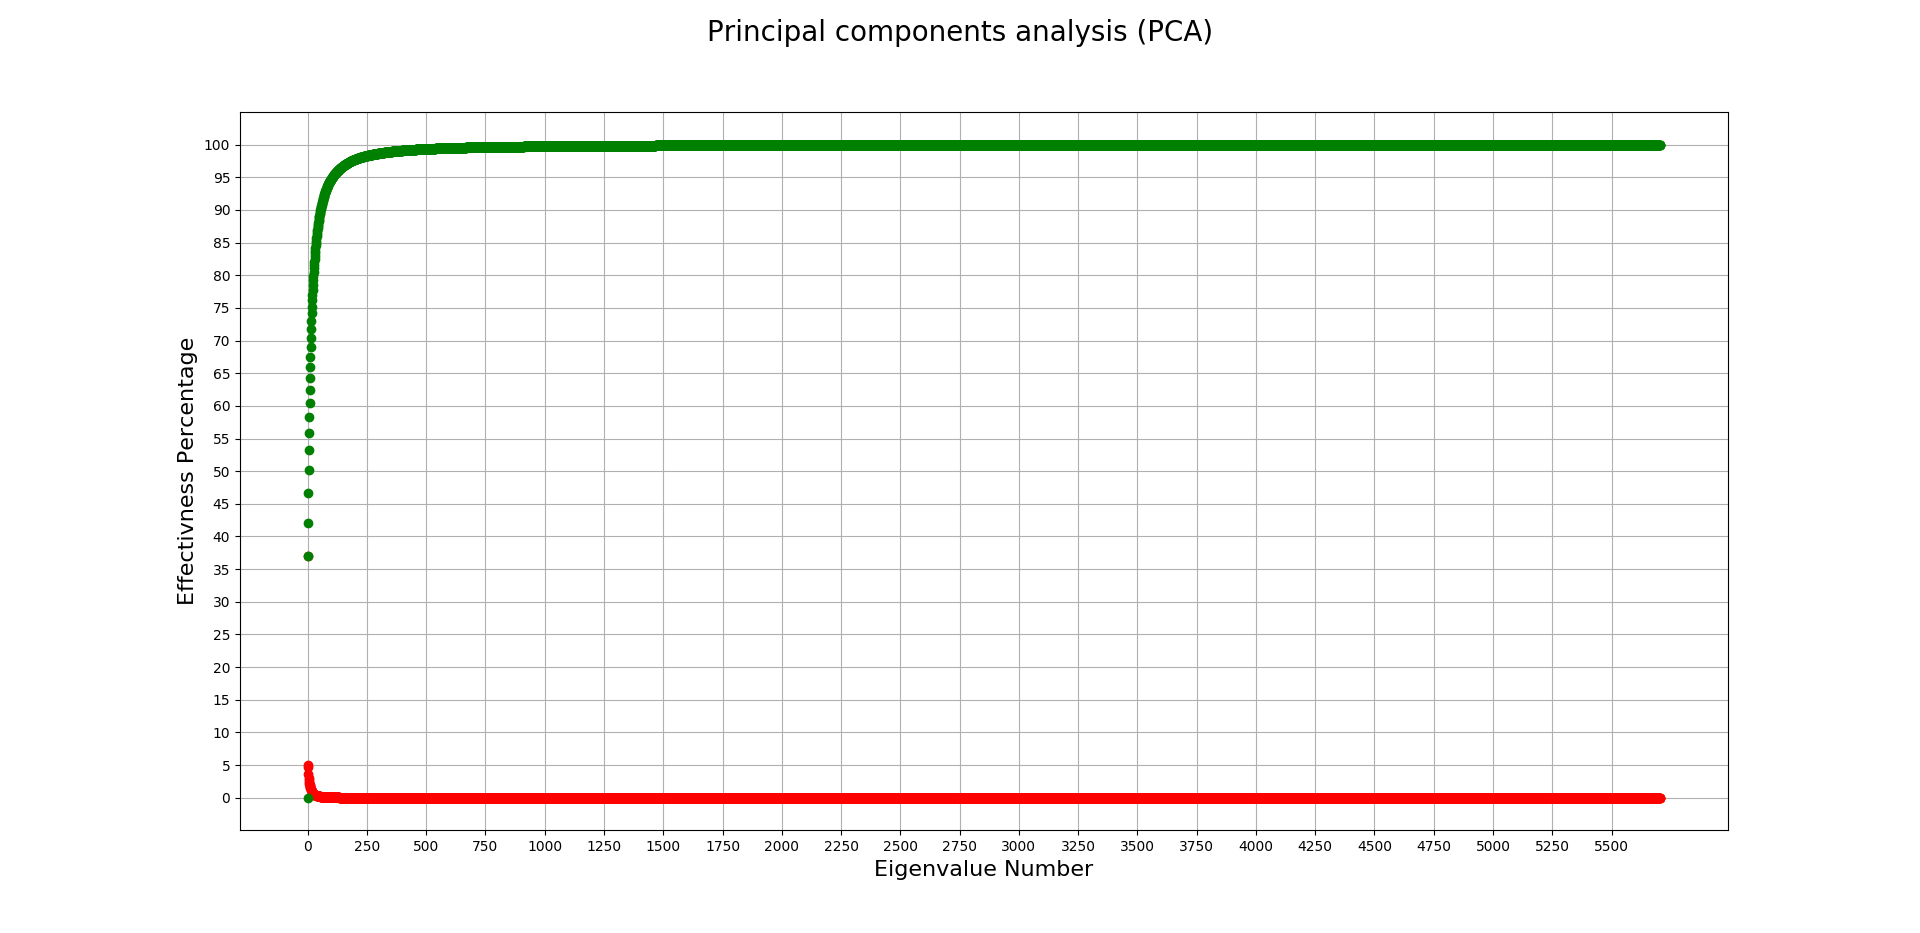
\includegraphics[scale=0.5]{kmeans_clustering/images/pca_grid}

Since we have 8300 words after removing for unique words it wasn't
possible to plot the PCA as a histogram. Even after removing all the
eigenvalues that were equal to zero we were left with thousands of
words. Instead we plotted only the non-zero eigenvalues as separate
points in a scatter plot. The eigenvalue are the red dots, for each
x-value there is an eigenvalue, and the scale is according to the
percentage of effectiveness of that eigenvalue. The green dots are
the cumulative values of the eigenvalues to that point.

We also tried to look at the PCA without removing words and got the
following:

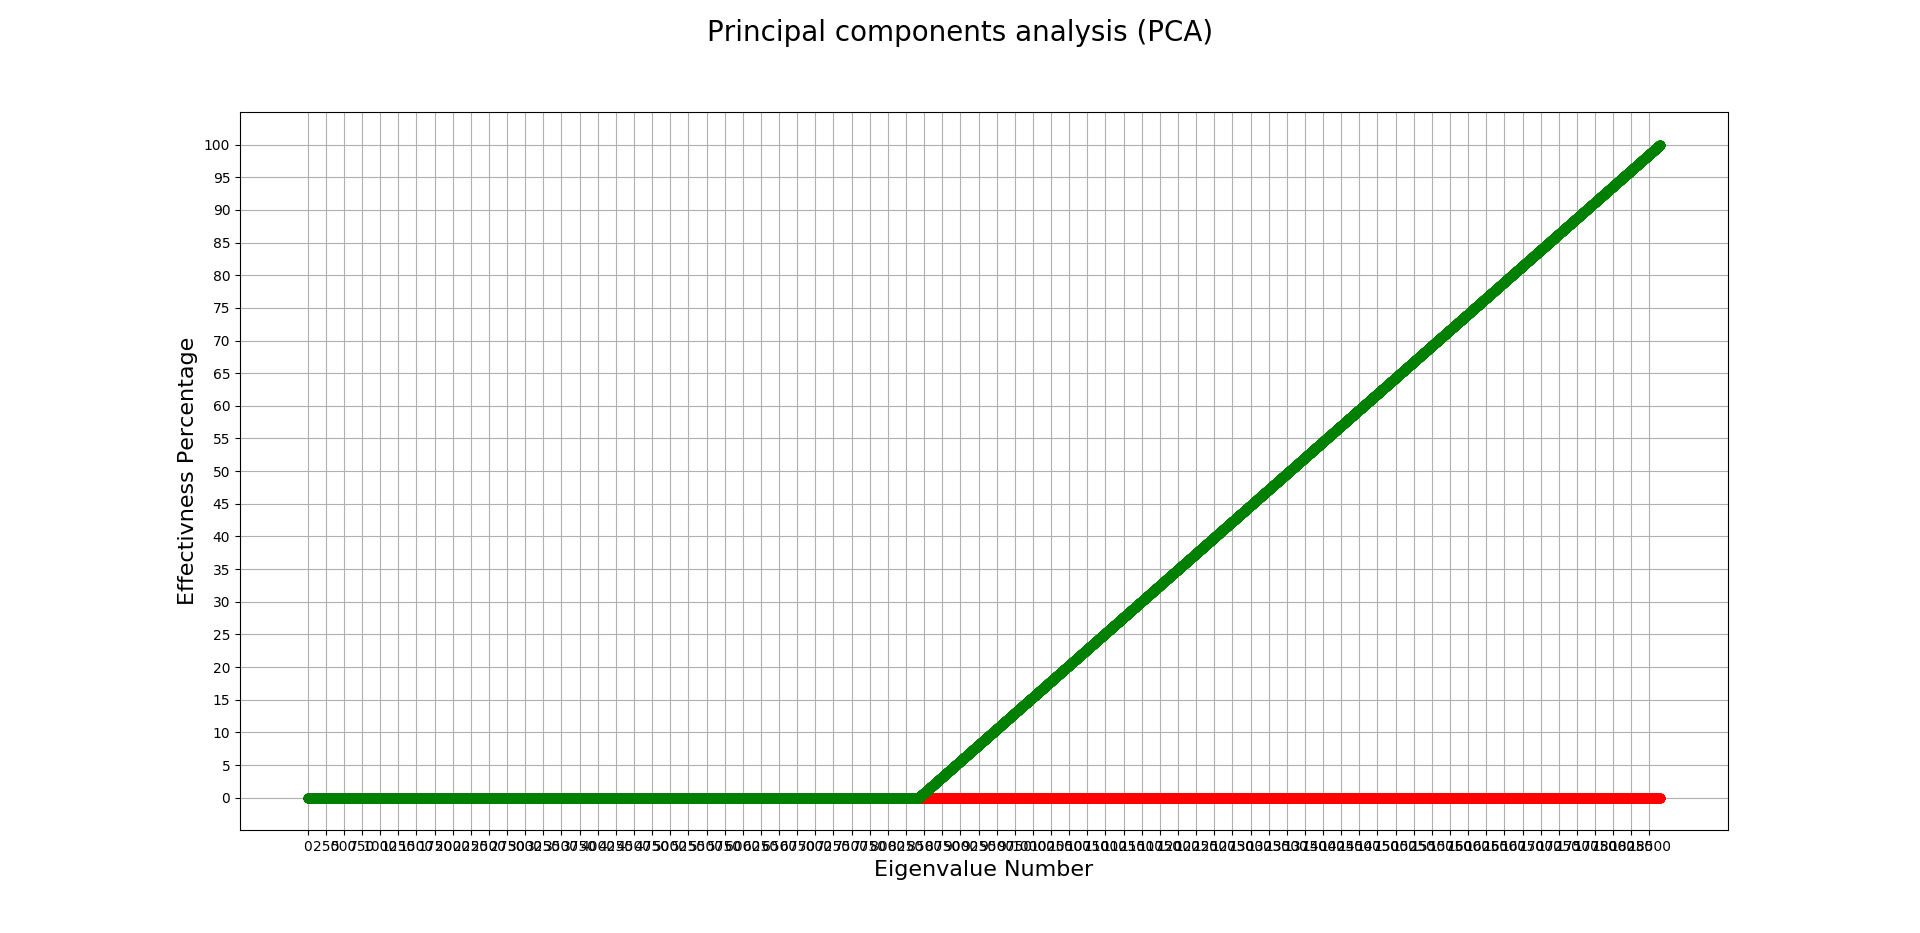
\includegraphics[scale=0.5]{kmeans_clustering/images/pca_all_words}

We can see that the values of all eigenvalues are roughly the same
and all very low, but accumulate because of the large number of them.
This supposedly means that all of the words are meaningful to the
same degree and should be kept, and was not very helpful to us.

We can see that around the 500th eigenvalue we start to have significant
stagnation, and after the 1500th eigenvalue we barely see any movement
at all. Thus we aimed at testing while setting our threshold variable
such that we would be left with 500 words and 1500 words to see what
results we would get, initially assuming that any more than 1500 words
wouldn't add any meaningful information.

\subsection{Results}

The best results we managed to get used the hyper-parameters:
\begin{itemize}
\item Amount of pages to be merged when reformatting the books = 10
\item k=7
\item removal = True
\item threshold for removing word = $0.4\cdot10^{-5}$
\end{itemize}
The results we obtained were:

\begin{lstlisting}
cluster 0 book_count: [0, 0, 0, 0, 0, 0, 0]
cluster 1 book_count: [5, 1, 0, 0, 0, 0, 0]
cluster 2 book_count: [1, 1, 1, 14, 106, 2, 14]
cluster 3 book_count: [0, 0, 0, 0, 0, 0, 0]
cluster 4 book_count: [28, 30, 2, 0, 0, 0, 0]
cluster 5 book_count: [0, 0, 0, 67, 5, 67, 71]
cluster 6 book_count: [1, 6, 46, 0, 0, 4, 0]
\end{lstlisting}

We can see a clear distinction between books 1,2,3 and books 4,5,6,7
as only clusters 2 and 6 has both groups represented, and the contrary
amount there is nearly negligible. Furthermore we can see that book
5 is relatively distinguishable from books 4,6 and 7, as cluster 2
focuses primarily on book 5 and cluster 5 focuses primarily on books
4,6, and 7. We can also see from clusters 1,4 and 6 that book 3 is
mostly distinguishable from books 1 and 2, but that books 1,2 aren't
easily separable.\\

It is interesting to see a clear gap between the first 3 books and
the later 4 books. This could have many different reasons, but a quick
search brought up that the first Harry Potter movie came out between
the time book 3 came out and book 4 came out, with a very unscientific
hunch we could assume it might of had an impact.\\

\subsection{Benchmark Dataset Results}

\subsection{First Attempt}

Previous to the current method of k-Means we attempted to process
the data in a different way. Initially we wanted to be able to graph
our data in a 2D plane in order to have it easily visualized. We devised
the following algorithm to process the words from the books left after
the removal stage and give them values on a 2D plane:

\begin{algorithm}

\caption{Initial attempt (words to 2D plane)}

\begin{lstlisting}
choose a word from dictionary - give it a value of 1.
for curr_word in dictionary do
	previous words values sum = 0
	for each word that already has a value do
		previous words values sum += \
			word value * amount that word appeared in all books together
	end for
	curr_word = previous words values sum + 1
end for
\end{lstlisting}
\end{algorithm}

This algorithm insured us a unique value for each word as well as
the fact that it was impossible to sum up different words and get
a value of another existing word (i.e. we could never have something
like ``harry'' + ``ron'' = ``hermione''). This is due to the
fact that each word in the dictionary is larger than the sum of all
instances of all the words before it. Thus given X words the sum of
those words is larger than the largest word in the input but smaller
than any word with a larger value than that of the largest word in
the input.

Another advantage of this was that by merely splitting up the initial
dictionary into N sub-dictionaries we could run this algorithm on
each sub-dictionary and thus get a representation of our data in any
N dimensions we wanted.\\

After some time of working with this algorithm for processing data
we realized that this method either arranges the pages in a completely
random way that cannot be clustered in any meaningful way, or we can
structure the data in a way that predefines the pages in clusters
- and thus any data we get is very biased and gives meaningless results.
This is due to the nature of the values we give the words: what ends
up happening is that when you give a value to a page for a dimension,
this value will be in between the value of the word with the largest
value in the page and the value of the word that is the next largest
in the sub-dictionary of this dimension (as explained above). Doing
this for each dimension of the domain would create ``boxes'' in
the domain that are exclusive to pages from a certain book. If we
randomize the order of the words on each axis, these ``boxes'' would
be located randomly on the board which essentially makes the domain
look like white noise. If we order the way the words get their values
on the axis (i.e. all words from book 1 get a smaller value than all
those from book 2, etc.) then we just artificially make the clusters
of pages of each book, and using k-means to cluster it will just cluster
our artificially made clusters and give meaningless results.

\subsection{Conclusion}

For the most part the results seem to show that differences between
the 7 books in the Harry Potter series can be found, and some books
can tend to be grouped together by the words that they use. This shows
that the use of the k-Means algorithm can be useful for analyzing
trends with time of word-based datasets. The k-Means algorithm is
relatively quick to compute and has little moving parts to adjust
(i.e. hyper-parameters) and as such provides an easy test bed for
testing out different theories via clustering. This being said k-Means
can also be very deceiving at times, and it is important to make sure
that the data processing is done with care and does not introduce
any biases.


\section{Hard Code}

\subsection{Background}

Hard coding is using the basic tools given in a programming language
to logic out an answer to a given problem. \\

After a while of trying different machine learning techniques we realized
that our data processing was manipulating the data in such a way that
just using a simple if statement in a couple of loops would probably
be able to solve the classification problem.This was due to the fact
that we were removing all words that weren't unique to a specific
book, thus all we needed to do is identify if one of the words that
were left over were in a given page, and knowing which book gave us
this word in the database in the first place we could then know which
book the page was from. \\

We also noticed that by choosing to keep unique words we were skewing
a bit from our initial goal of discovering writing patterns and ended
up just identifying pages via new character names or objects or places
from the different books. Looking at it from this aspect makes it
seem much more like a simple problem that can be hard coded.

\subsection{Methods}

\subsubsection{Data Pre-Processing}

For data processing we did the exact same thing done in the data processing
for k-Means (see \ref{subsec:kMeans-Data-Processing}) up to the point
of merging pages. The only thing to note is that we chose a threshold
of 0 while removing data (thus keeping all of the words that were
unique per a single book).

\subsubsection{Hard Coding Procedure}

The algorithm used is a follows:

\begin{algorithm}

\caption{Hard Coding}

\begin{lstlisting}
total classifications = 0
correct classifications = 0
for each book:
	for each page in the book:
		total classifications += 1
		for each word in our database:
			if the word is in the book:
				if the page came from the same book the word came from:
					correct classifications += 1
					go to testing next page
		if the page did not contain any word for the database:
			randomly choose a book
result = correct classifications / total classifications		
\end{lstlisting}
\end{algorithm}

There are improvements that can be made to this algorithm, such as
taking semi unique words into account, but we found the results we
got were good enough to prove our point and it was unnecessary to
continue tinkering.

\subsubsection{Hyper-Parameter Tuning}

The only hyper-parameter we could tune was:
\begin{itemize}
\item The amount of pages to be merged
\end{itemize}
We chose to keep this at 1 (thus not merging any pages) as this would
give us the least probability to find a unique word, and thus is the
hardest case. If this would give us a good result then that would
be the strongest statement possible.

\subsection{Results}

Using this method we managed to get 99.63\% accuracy (4683/4700 pages
correctly classified). In case we just got lucky with our random picks
we also tried to run the algorithm without a random pick of a book
if no unique words were found in a page, and that gave use 95.59\%
accuracy (4681/4700 pages correctly classified). These results were
also obtained significantly faster than any of our machine learning
methods, as the computation time could be counted in a few seconds
as apposed to several minutes for the other methods\\

As mentioned earlier if we were to merge more pages, or take semi-unique
words into account we could probably improve upon this result, but
we felt that the results were good enough to make our point.

\subsection{Conclusions}

Machine learning is cool, but can sometimes over-complicate a problem.
If you find yourself going down a rabbit hole - Occam's razor can
save you a lot of time, energy and frustration. That being said, the
different techniques did give us some insight that we could not obtain
using the hard coding method, such as which books appear more similar
and around which books did J.K Rowling start using more different
words.

\section{Final Thoughts}


\end{document}
